\setlength{\baselineskip}{20pt}
\chapter{Relevant Theories on Metal Superhydrophobic Surface}
\label{cha:chap2}

\section{Classical theoretical model of wettability}

\subsection{Young model}


\begin{figure}[!htb] % use float package if you want it here
%\setlength{\abovecaptionskip}{-0.2cm} %调整图片caption与正文之间的间距，table同理。可自己调整。
\setlength{\belowcaptionskip}{-0.2cm} 
  \centering
  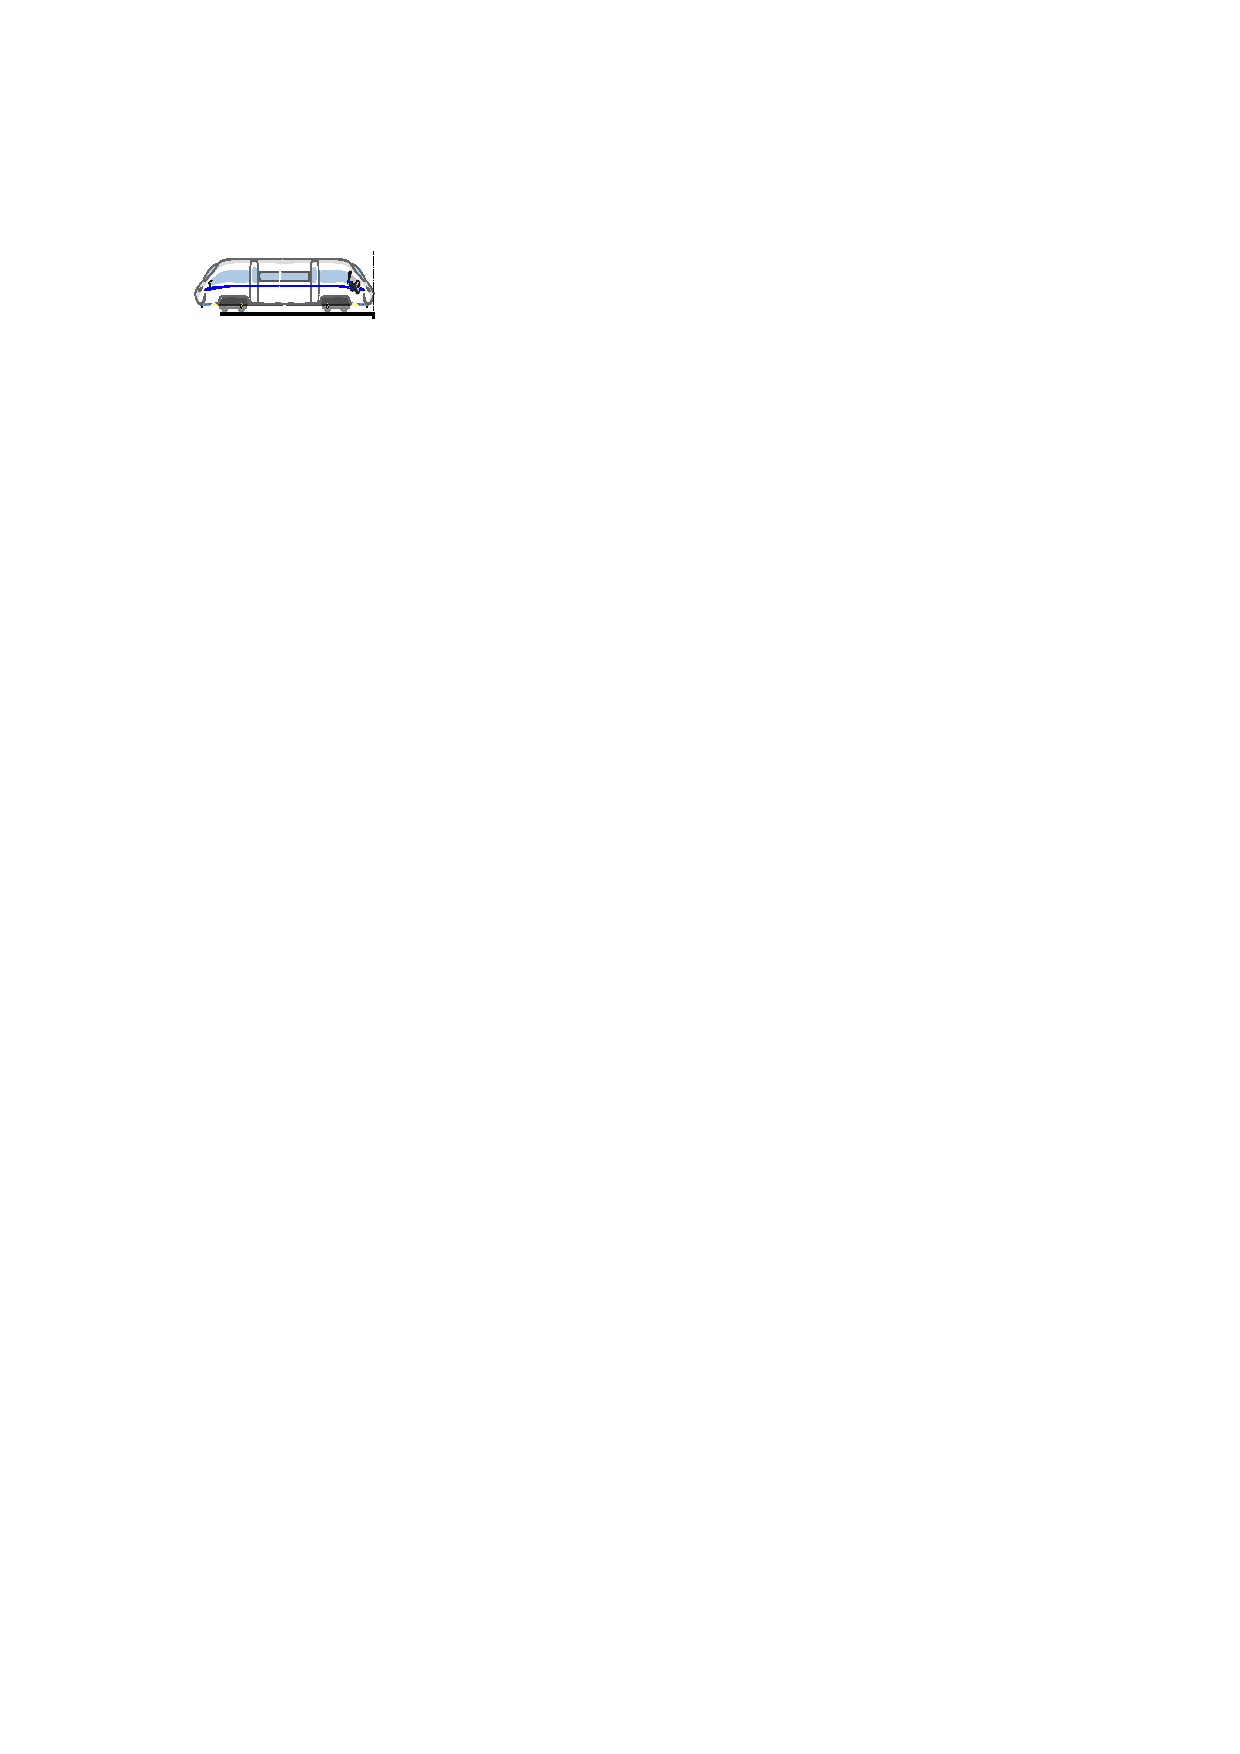
\includegraphics[scale=1]{figures/figure1.pdf}
  \caption{示例图片。}
  \label{fig:02:01}
\end{figure}


例如：如表格\ref{table:02:01}所示

\begin{table}[!htb]\small   %%\small是为了设置表格中的字体比正文小
\setlength{\abovecaptionskip}{-0.05cm} %调整图片caption与正文之间的间距，table同理。可自己调整。
\setlength{\belowcaptionskip}{-0.2cm} 
  \centering
  \renewcommand\arraystretch{1}
  \caption{示例表格。}

 \begin{tabular}{p{1cm} p{1cm}<{\centering} p{1cm}<{\centering} p{1cm}<{\centering} p{1cm}<{\centering} p{1cm}<{\centering}  }
  \hline
  AA &
  BB &
  CC &
  DD &
  EE &
  FF
  \\
  \hline
    AA   &  1.1   & 1.1 & 1.1 & 1.1&  1.1    \\
    BB   &  1.1   & 1.1 & 1.1 & 1.1&  1.1    \\
    CC   &  1.1   & 1.1 & 1.1 & 1.1&  1.1   \\
  \hline
  \end{tabular}
  \label{table:02:01}
\end{table}


单独为行公式示例：如公式\ref{eq:02:01}，公式\ref{eq:02:02a}所示。

\begin{equation}\label{eq:02:01}
\left\{
\begin{split}
\frac{\texttt{d}p(t)}{\texttt{d}t}&=v(t)\\
\frac{\texttt{d}v(t)}{\texttt{d}t}&=u(t)-a(t)-b(t)v(t)-c(t)v^2(t)-f_2^*(\cdot)
\end{split}
\right.
\end{equation}


\begin{subequations}\label{eq:02:02}
  \begin{align}
  \dot{\hat{A}}^\dag&=\lambda_1\left(\tanh(k_3e_v)e_v-\sigma_1\hat{A}^\dag\right)\label{eq:02:02a}\\
  \dot{\hat{b}}^\dag&=\lambda_2\left(|v||e_v|-\sigma_2\hat{b}^\dag\right)\label{eq:02:02b}\\
  \dot{\hat{c}}^\dag&=\lambda_3\left(v^2|e_v|-\sigma_3\hat{c}^\dag\right)\label{eq:02:02c}
  \end{align}
  \end{subequations}

嵌入在文本中的公式例子：$a + b = c$。

\subsection{Wenzel model}

\subsection{Cassie-Baxter model}

\section{Summary}




%\bibliography{reference/ref.bib}


